\chapter{Estado del arte}
En este capítulo se hablará sobre los dos conceptos que funcionan como base del proyecto, que son SDN y NFV.

Así mismo, se hará una breve introducción a Net2Plan, que es la herramienta open-source en la que se basa la herramienta desarrollada.

Por último, se hablará de las diferentes herramientas/aplicaciones que se han utilizado para llevar a cabo este proyecto, como pueden ser ONOS, ETSI-OSM y OpenStack, y de las librerías JAVA que se han empleado para poder realizar la interacción entre todos los componentes.


\section{Herramientas Open-Source en entornos de red}
\label{sec:opensourceentornored}

\section{Redes de transporte}
\label{sec:redestransporte}

\section{SDN}
\label{sec:sdn}

\begin{figure}[!ht]
	\centering
	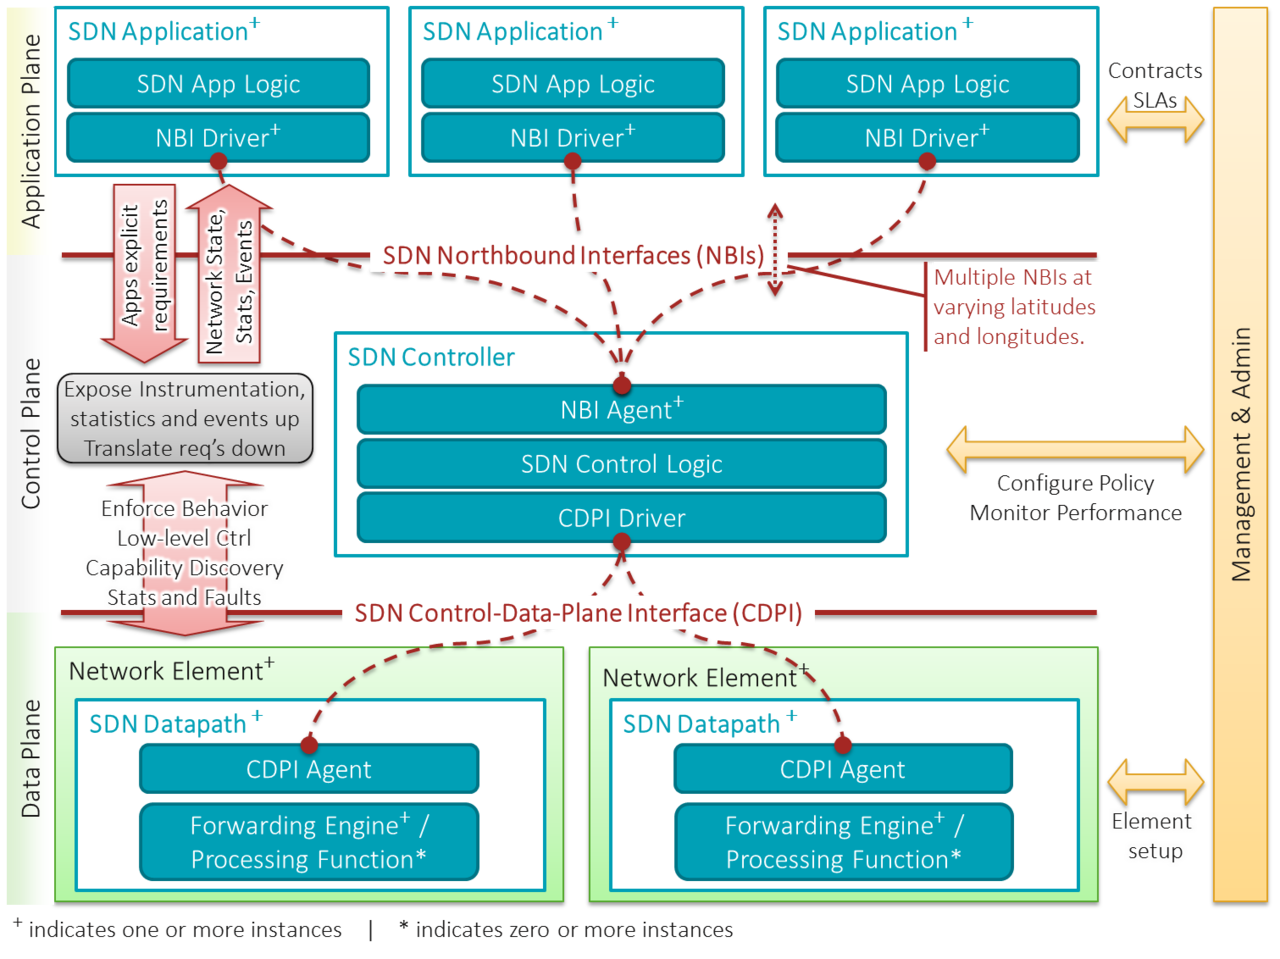
\includegraphics[width=0.75\linewidth]{imagenes/arquitectura_sdn}
	\caption{Arquitectura SDN}
	\label{fig:arquitecturasdn}
\end{figure}

\subsection{OpenFlow}
\label{subsec:openflow}

\section{NFV}
\label{sec:nfv}


\cleardoublepage